\subsection{Sprint 3}

\subsubsection{Logical Lines Of Code (LLOC)}
\label{section:sprint3LLOC}

\begin{figure}
\centering
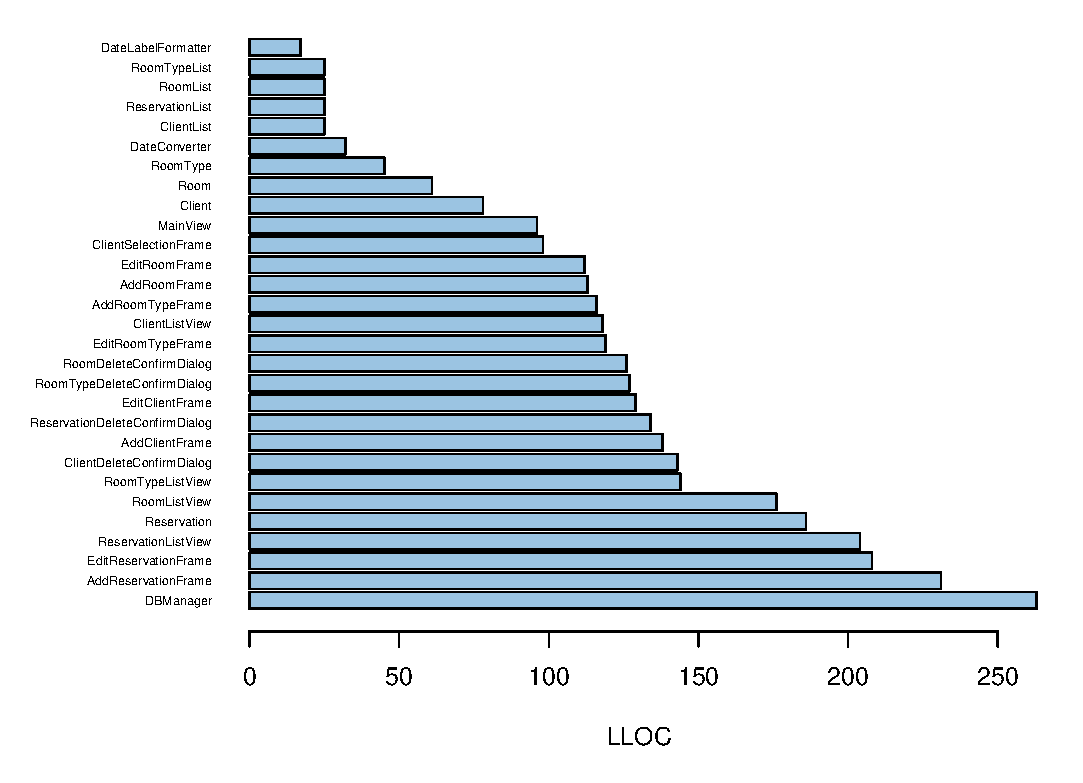
\includegraphics[width=1.0\textwidth]{Sprint3-LLOC-1.eps}
\caption{Λογικές γραμμές κώδικα ανά κλάση στο τέλος του sprint 3}
\label{fig:sprint3LLOC}
\end{figure}

\subsubsection{Clone Coverage (CC)}
\label{section:sprint3CC}

\begin{figure}
\centering
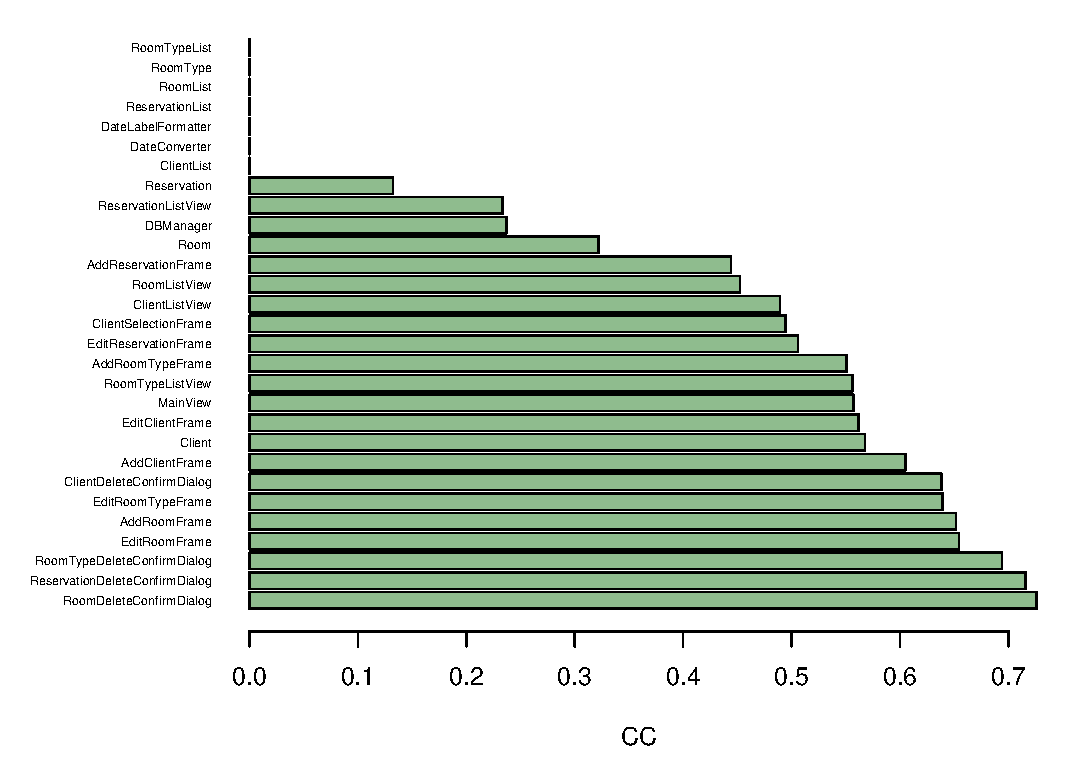
\includegraphics[width=1.0\textwidth]{Sprint3-CC-1.eps}
\caption{Τιμές της μετρικής CC ανά κλάση στο τέλος του sprint 3}
\label{fig:sprint3CC}
\end{figure}

\subsubsection{McCabe’s Cyclomatic Complexity (McCC)}
\label{section:sprint3McCC}

\begin{figure}
\centering
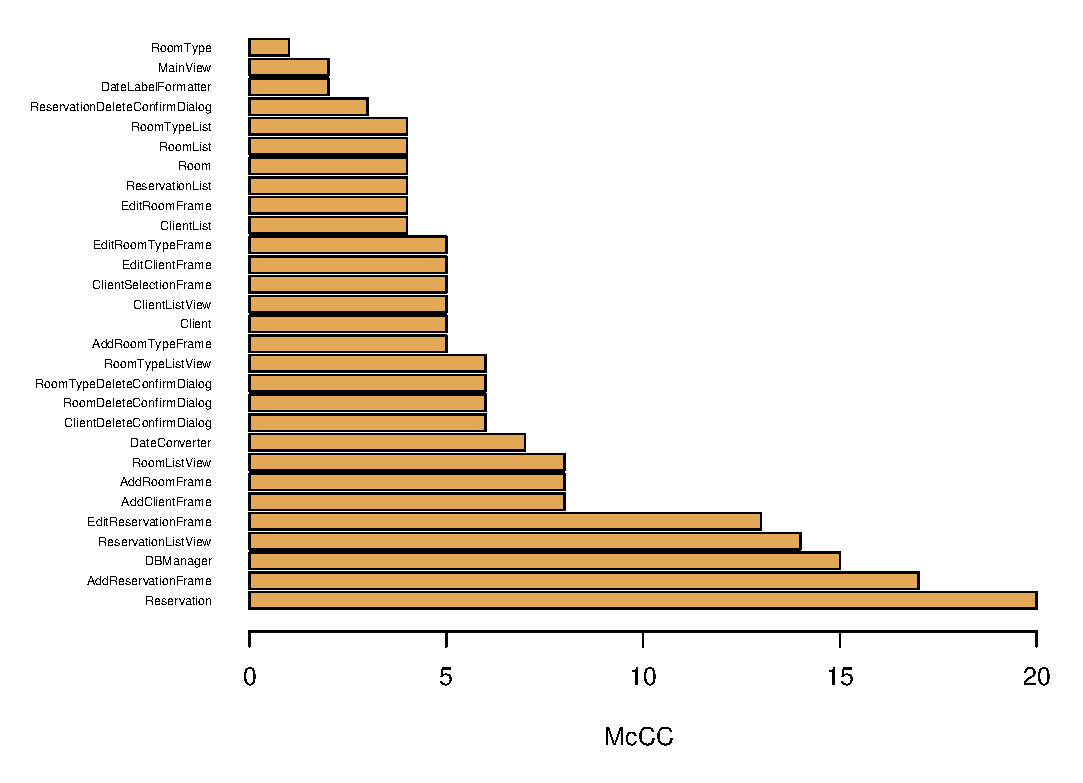
\includegraphics[width=1.0\textwidth]{Sprint3-McCC-1.eps}
\caption{Τιμές της μετρικής κυκλωματικής πολυπλοκότητας McCC ανά κλάση στο τέλος του sprint 3}
\label{fig:sprint3McCC}
\end{figure}

\subsubsection{Lack of Cohesion in Methods 5 (LCOM5)}
\label{section:sprint3LCOM5}

\begin{figure}
\centering
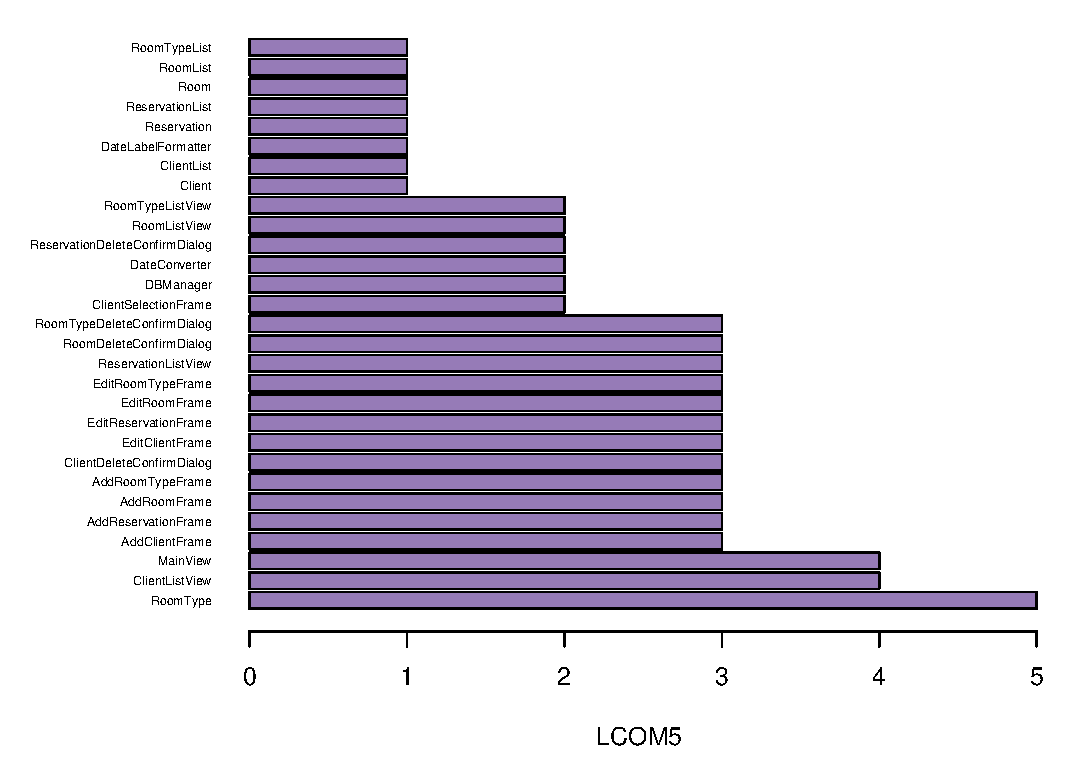
\includegraphics[width=1.0\textwidth]{Sprint3-LCOM5-1.eps}
\caption{Τιμές της μετρικής έλλειψης συνεκτικότητας LCOM5 ανά κλάση στο τέλος του sprint 3}
\label{fig:sprint3LCOM5}
\end{figure}

\subsubsection{Coupling Between Object classes (CBO)}
\label{section:sprint3CBO}

\begin{figure}
\centering
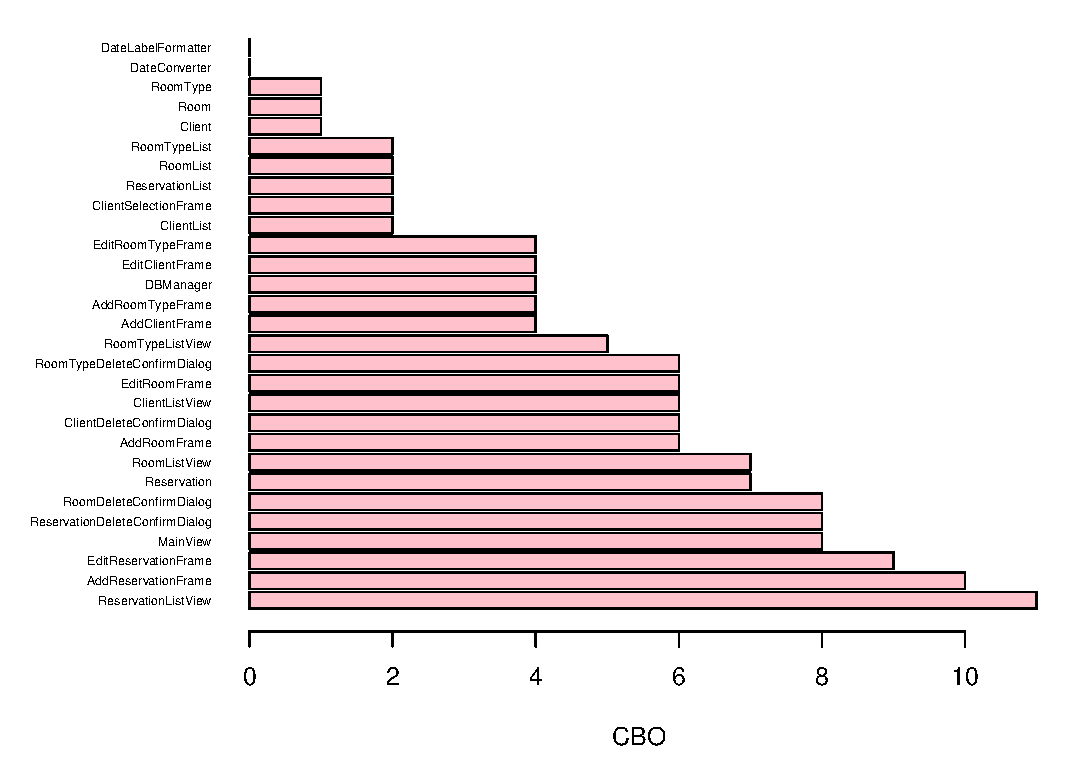
\includegraphics[width=1.0\textwidth]{Sprint3-CBO-1.eps}
\caption{Τιμές της μετρικής σύζευξης CBO ανά κλάση στο τέλος του sprint 3}
\label{fig:sprint3CBO}
\end{figure}
